\begin{flushright} {\tiny {\color{gray} continuum\_mechanics.tex}} \end{flushright}
%~~~~~~~~~~~~~~~~~~~~~~~~~~~~~~~~~~~~~~~~~~~~~~~~~~~~~~~~~~~~~~~~~~~~~~~~~~~~~~~~~~~~~~~~~~~~~~~~~~

{\sl Contains contributions by W. Spakman - Continuum mechanics course syllabus} 
\index{contributors}{W. Spakman}

%......................................................................
\subsubsection{Forces}

In continuum mechanics we make a distinction between two broad classes of forces:
\begin{itemize}
\item Body forces defined as force per unit volume (\si{\newton\per\cubic\metre}): 
gravity, electro-magnetic forces
\item Tractions: Surface forces defined as force per unit surface area (\si{\newton\per\square\metre}):
Contact forces, elastic forces per unit area, internal flow friction, pressure, ...\\
A traction is the surface average of all atomic forces exerted by
atoms on the one side on atoms on the other side of the surface.
For real-Earth processes, internal tractions are ultimately caused by
the body forces, usually gravity.


Existing mantle flow(i.e. flow that is forced elsewhere) can exert
tractions (shear stresses) on the subducting slab or for instance at
the base of lithosphere plates.
In HPT-laboratory experiments external tractions (pressure, shear
traction) are applied to a rock sample, which cause internal
tractions to balance the exerted forces.

\begin{center}
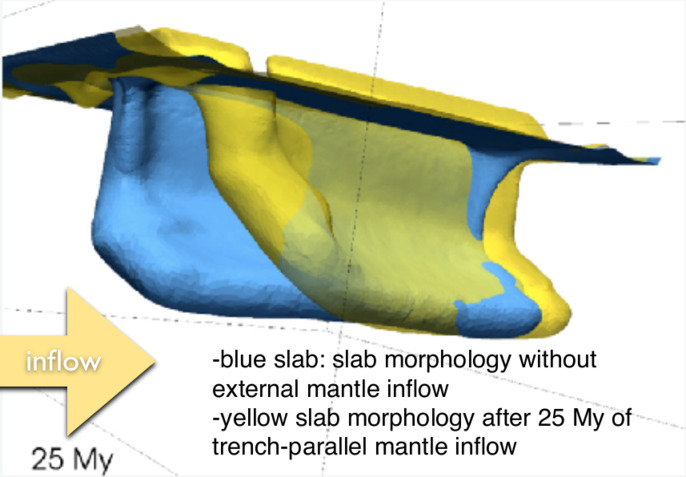
\includegraphics[width=6cm]{images/contmech/spak1}
\end{center}
\end{itemize}

%......................................................................
\subsubsection{Stress tensor and tractions}\label{sec:stresstensor}
\index{general}{Stress Tensor} 
\index{general}{Normal Stress} 
\index{general}{Shear Stress} 
\index{general}{Stress Vector} 
\index{general}{Traction}

The Cauchy stress tensor\footnote{\url{https://en.wikipedia.org/wiki/Cauchy_stress_tensor}} 
consists of nine components $\sigma_{ij}$  that completely define the state of stress 
at a point inside a material. 
The tensor relates a unit-length direction vector $\vec{n}$ to the so-called 'stress vector' (most commonly called 'traction') $\vec{t}(\vec{n})$ across an imaginary surface perpendicular to $\vec{n}$:
\[
\vec{t}(\vec n)= {\bm \sigma}\cdot {\vec n}
\]

\begin{center}
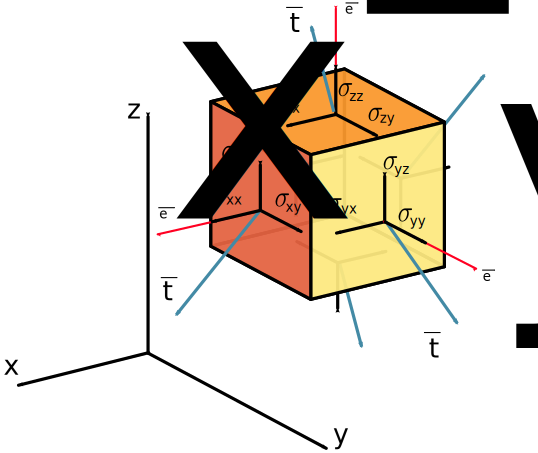
\includegraphics[width=7cm]{images/contmech/Components_stress_tensor_cartesian}\\
{\scriptsize Modified from original 
file on Wikipedia\footnote{\url{https://commons.wikimedia.org/wiki/File:Components_stress_tensor_cartesian.svg}}}
\end{center}

\noindent 
With respect to an orthonormal basis $\{\vec{e}_x,\vec{e}_y,\vec{e}_z\}$, the Cauchy stress tensor
is given by:
\begin{equation}
{\bm \sigma}=
\left(
\begin{array}{ccc}
\sigma_{xx} & \sigma_{xy} & \sigma_{xz} \\
\sigma_{yx} & \sigma_{yy} & \sigma_{yz} \\
\sigma_{zx} & \sigma_{zy} & \sigma_{zz} 
\end{array}
\right)
\end{equation}
The three diagonal elements are called normal stresses while the off-diagonal terms 
are called shear stresses.

One can easily prove (see for instance Section 3.3.6 of \cite{grbl09}) that the balance 
of angular momentum leads reduces to the statement that the Cauchy stress tensor 
is symmetric, i.e. ${\bm \sigma}={\bm \sigma}^T$.
Therefore, the stress state of the medium at any point and instant can be specified by only six independent parameters, rather than nine:
\begin{equation}
{\bm \sigma}=
\left(
\begin{array}{ccc}
\sigma_{xx} & \sigma_{xy} & \sigma_{xz} \\
\sigma_{xy} & \sigma_{yy} & \sigma_{yz} \\
\sigma_{xz} & \sigma_{yz} & \sigma_{zz} 
\end{array}
\right)
\qquad\qquad
\text{or sometimes}
\qquad\qquad
{\bm \sigma}=
\left(
\begin{array}{ccc}
\sigma_{x}  & \tau_{xy}  & \tau_{xz} \\
\tau_{xy}   & \sigma_{y} & \tau_{yz} \\
\tau_{xz}   & \tau_{yz}  & \sigma_{z} 
\end{array}
\right)
\end{equation}
where the elements $\sigma _{x}$, $\sigma _{y}$, $\sigma _{z}$ are called the orthogonal 
normal stresses (relative to the chosen coordinate system), and $\tau _{xy}$, $\tau _{xz}$,
$\tau _{yz}$ the orthogonal shear stresses. The left form is preferred in this document.
As seen above, the SI units of both stress tensor and traction are \si{\newton\per\square\metre}.

\todo[inline]{specify the underlying assumptions in what follows}

In Cylindrical coordinates the stress tensor components are given by:
\begin{eqnarray}
\sigma_{rr} &=& -p + 2 \eta \frac{\partial \upnu_r}{\partial r}      \\
\sigma_{\theta\theta} &=& 
 -p + 2\eta \left( \frac{1}{r} \frac{\partial \upnu_\theta}{\partial\theta} +\frac{\upnu_r}{r} \right)    \\
\sigma_{zz} &=& -p + 2 \eta \frac{\partial \upnu_z}{\partial z}      \\
\sigma_{r\theta} &=& \eta \left( \frac{1}{r} \frac{\partial \upnu_r}{\partial \theta} 
+ \frac{\partial \upnu_\theta}{\partial r} - \frac{\upnu_\theta}{r} \right)  \\
\sigma_{rz} &=& \eta \left( \frac{\partial \upnu_r}{\partial z}  + \frac{\partial \upnu_z}{\partial r}\right) \\
\sigma_{\theta z} &=&  \eta \left(  \frac{1}{r} \frac{\partial \upnu_z}{\partial \theta}
+\frac{\partial \upnu_\theta}{\partial z}     \right) 
\end{eqnarray}
\index{general}{Stress Tensor (Cylindrical Coordinates)}

In Spherical coordinates the stress tensor components are given by:
\begin{eqnarray}
\sigma_{rr} &=& -p + 2 \eta \frac{\partial \upnu_r}{\partial r}      \\
\sigma_{\theta\theta} &=& 
 -p + 2\eta \left( \frac{1}{r} \frac{\partial \upnu_\theta}{\partial\theta} +\frac{\upnu_r}{r} \right)    \\
\sigma_{\phi\phi} &=& 
-p + 2\eta \left( \frac{1}{r \sin \theta} \frac{\partial \upnu_\phi}{\partial \phi} 
+\frac{\upnu_r}{r}  + \frac{\upnu_\theta \cot \theta}{r} \right) \\
\sigma_{r\theta} &=& \eta\left(  r \frac{\partial}{\partial r} \frac{\upnu_\theta}{r}  
+\frac{1}{r} \frac{\partial \upnu_r}{\partial\theta}   \right)\\
\sigma_{r\phi} &=& \eta \left( \frac{1}{r \sin\theta}\frac{\partial \upnu_r}{\partial \phi} 
+ r \frac{\partial}{\partial r} \frac{\upnu_\phi}{r}  \right)\\
\sigma_{\theta \phi} &=& \eta \left(
\frac{1}{r \sin\theta} \frac{\partial \upnu_\theta}{\partial\phi}
+\frac{\sin\theta}{r} \frac{\partial}{\partial \theta} \frac{\upnu_\phi}{\sin\theta}
\right) 
\end{eqnarray}
\index{general}{Stress Tensor (Spherical Coordinates)}



